\documentclass[11pt,a4paper]{article}

\usepackage[margin=2.5cm]{geometry}
\usepackage{graphicx}
\usepackage{amsmath,amssymb}
\usepackage{booktabs}
\usepackage{hyperref}
\usepackage{subcaption}
\usepackage{float}
\usepackage{enumitem}
\usepackage[numbers,sort&compress]{natbib}

\hypersetup{
  colorlinks=true,
  linkcolor=blue,
  citecolor=blue,
  urlcolor=blue
}

\title{\textbf{MNIST Generative Models Lab:\\From Manual Classifiers to VAE, DDPM, and GANs}}
\author{Technical report (portfolio project)\\
  \texttt{mnist-generative-models-lab}}
\date{July 2026}

\begin{document}
\maketitle

\begin{abstract}
I built a notebook-driven MNIST lab with two tracks: classification (from-scratch KNN and logistic regression through a PyTorch CNN) and generation (VAE, pixel-space DDPM, DCGAN, and a latent diffusion MLP). On the saved notebook outputs I kept, test accuracy climbs from \textbf{0.9705} (GPU KNN, $k{=}3$) to \textbf{0.9913} (comparison CNN), with logistic regression sitting lower at \textbf{0.9241} because it is strictly linear. The generative notebooks train end-to-end and produce readable digit samples, but I did not compute FID or Inception Score; my conclusions about sample quality are qualitative, based on the PNGs exported to \texttt{results/figures/}. I document both what worked as a learning path and what I would refactor next (duplicate VAE training, misleading notebook filename, missing quantitative generative metrics).
\end{abstract}

\section{Introduction}
\label{sec:intro}

I chose MNIST~\citep{lecun1998gradient} because it is the standard place to make model behaviour visible before scaling up. This repo is not a production system; it is a curriculum I can walk through in Jupyter: understand the data, implement classical models by hand, add a small CNN, benchmark everything side by side, then explore compression (VAE), denoising (DDPM), adversarial training (DCGAN), and finally diffusion in a 16-D latent space.

Figure~\ref{fig:roadmap} shows the order I used. Each notebook preserves embedded outputs so metrics and plots are inspectable without retraining. All figures in this report were copied from those outputs into \texttt{results/figures/}; I did not regenerate checkpoints from gitignored \texttt{training\_results/} or \texttt{*.pth} files.

\begin{figure}[H]
  \centering
  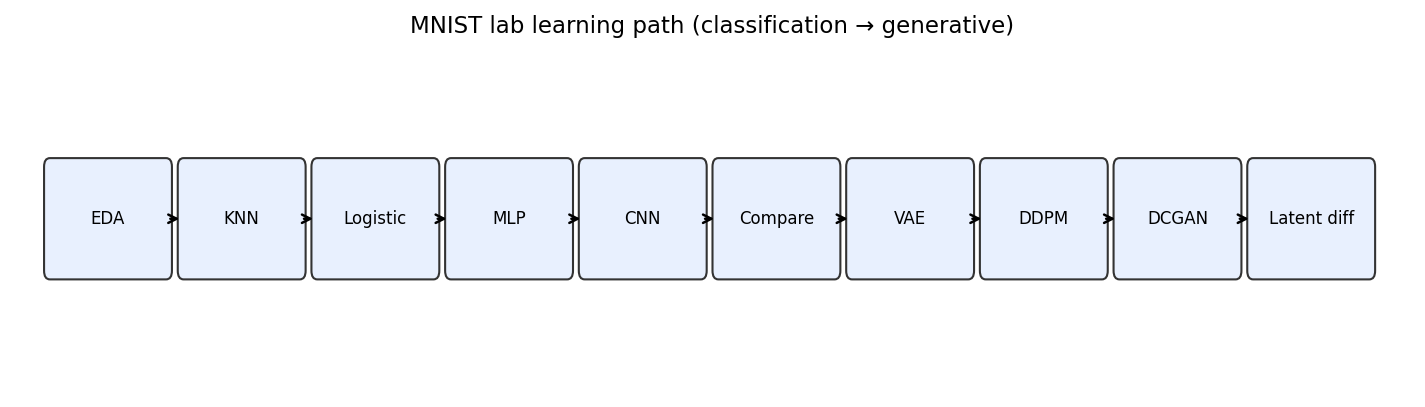
\includegraphics[width=0.98\textwidth]{../results/figures/00_roadmap/learning_path.png}
  \caption{Learning path I followed: EDA $\rightarrow$ manual classifiers $\rightarrow$ CNN $\rightarrow$ multi-model comparison $\rightarrow$ generative models.}
  \label{fig:roadmap}
\end{figure}

\section{Exploratory data analysis}
\label{sec:eda}

Before training anything, \texttt{eda\_analysis.ipynb} loads MNIST and walks through class balance, per-digit galleries, mean templates, pixel variance maps, intensity histograms, and PCA structure. On visual inspection, the class counts are nearly even (Figure~\ref{fig:balance}), which means raw accuracy is a reasonable metric and I do not need heavy rebalancing tricks for this dataset.

\begin{figure}[H]
  \centering
  \begin{subfigure}[b]{0.48\textwidth}
    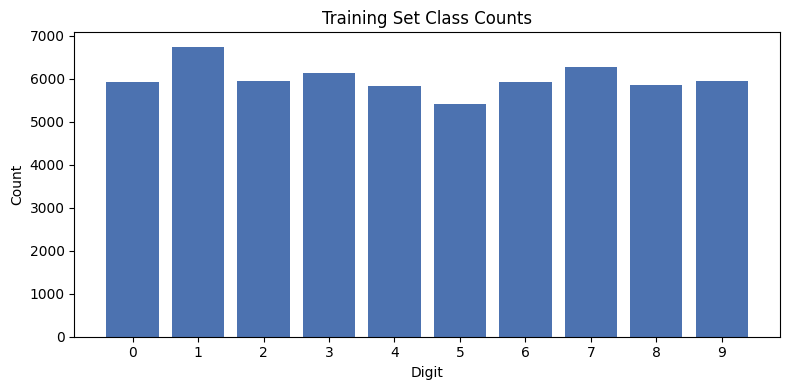
\includegraphics[width=\textwidth]{../results/figures/01_eda/class_balance.png}
    \caption{Class balance}
    \label{fig:balance}
  \end{subfigure}
  \hfill
  \begin{subfigure}[b]{0.48\textwidth}
    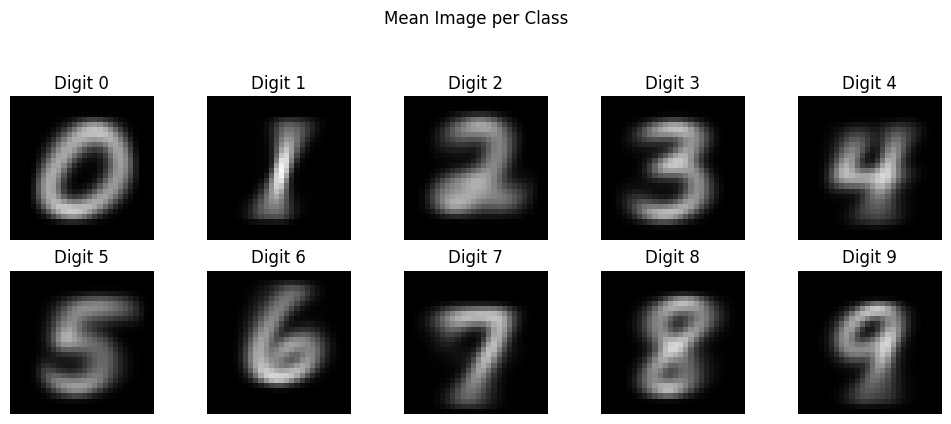
\includegraphics[width=\textwidth]{../results/figures/01_eda/mean_digits.png}
    \caption{Mean digit templates}
    \label{fig:mean}
  \end{subfigure}
  \caption{EDA findings from my saved notebook run. Digits are centred and stroke thickness varies by class.}
  \label{fig:eda}
\end{figure}

The mean images (Figure~\ref{fig:mean}) look like the digits I expect, but PCA plots (Figure~\ref{fig:pca}) show substantial overlap between classes in the first two components. That overlap is my main motivation for non-linear models: a single linear boundary in pixel space cannot separate all ten digits cleanly, even though MNIST is ``easy'' by modern standards.

\begin{figure}[H]
  \centering
  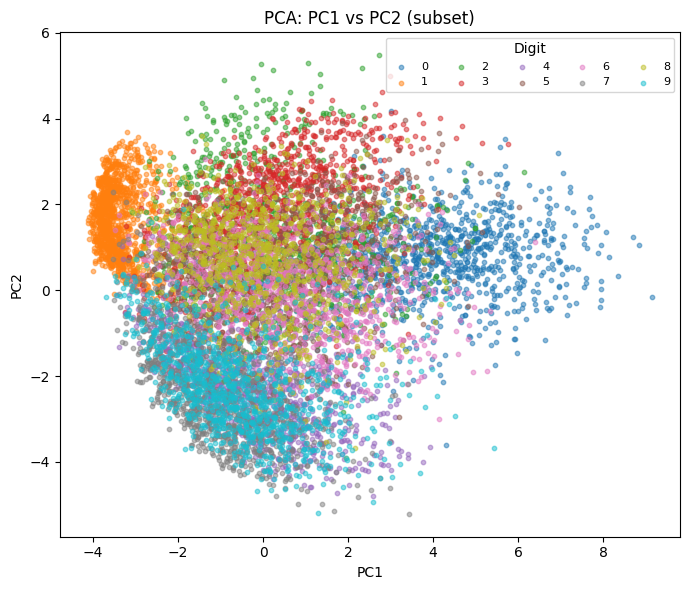
\includegraphics[width=0.65\textwidth]{../results/figures/01_eda/pca_overlap.png}
  \caption{PCA structure in the training set. Classes overlap in low-dimensional projections, which foreshadows linear-model limits.}
  \label{fig:pca}
\end{figure}

\section{Classical and manual machine learning}
\label{sec:manual}

\subsection{KNN and the bias--variance tradeoff}

In \texttt{manual\_knn.ipynb} I implemented KNN in NumPy and then batched it on GPU with \texttt{torch.cdist}. A sweep over $k \in \{1,3,5,9,15,20\}$ (Figure~\ref{fig:knn}) shows accuracy peaking near $k{=}3$ at \textbf{0.9705} on the full test set. Very small $k$ is noisier; very large $k$ oversmooths decision boundaries. I found this plot more instructive than the final scalar accuracy because it makes the tradeoff concrete.

\begin{figure}[H]
  \centering
  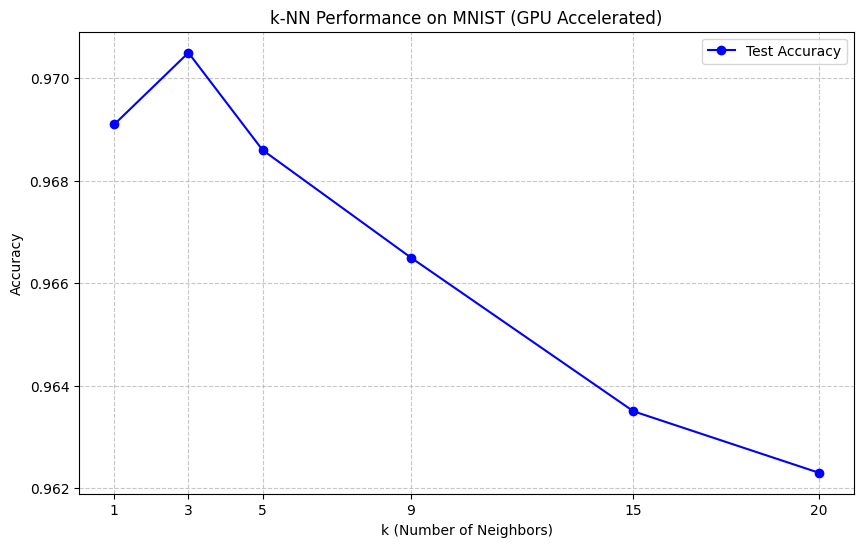
\includegraphics[width=0.72\textwidth]{../results/figures/02_knn/k_sweep.png}
  \caption{GPU KNN accuracy vs.\ $k$ from my notebook outputs.}
  \label{fig:knn}
\end{figure}

\subsection{Logistic regression: a deliberate dip in the ladder}

I expected accuracy to improve monotonically as models gained capacity. That did not happen. My from-scratch softmax regression in \texttt{manual\_logistic\_reg.ipynb} plateaus at \textbf{0.9241}, below KNN and well below the manual MLP. I think that is mostly a capacity issue: logistic regression is a linear classifier in pixel space, and MNIST digits written in different styles still overlap when flattened to 784 dimensions. Figure~\ref{fig:misclass} shows the kind of errors I get---confusions between visually similar strokes (e.g.\ 4 vs 9, 3 vs 5).

\begin{figure}[H]
  \centering
  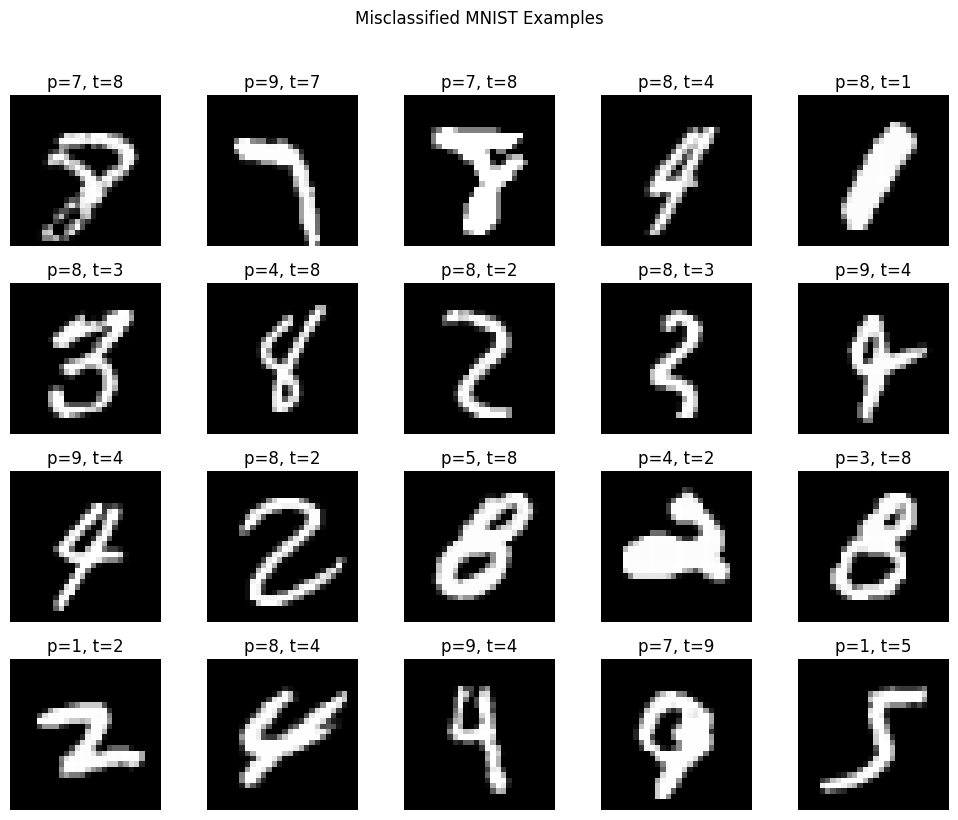
\includegraphics[width=0.85\textwidth]{../results/figures/03_logistic/misclassified_grid.png}
  \caption{Misclassified test digits from my logistic regression run.}
  \label{fig:misclass}
\end{figure}

\subsection{Manual MLP}

Adding one ReLU hidden layer ($H{=}128$, 100 epochs) in \texttt{manual\_mlp.ipynb} raised accuracy to \textbf{0.9794}. The first-layer weight templates (Figure~\ref{fig:mlp}) look like crude stroke detectors; that made backprop feel less abstract than reading equations alone.

\begin{figure}[H]
  \centering
  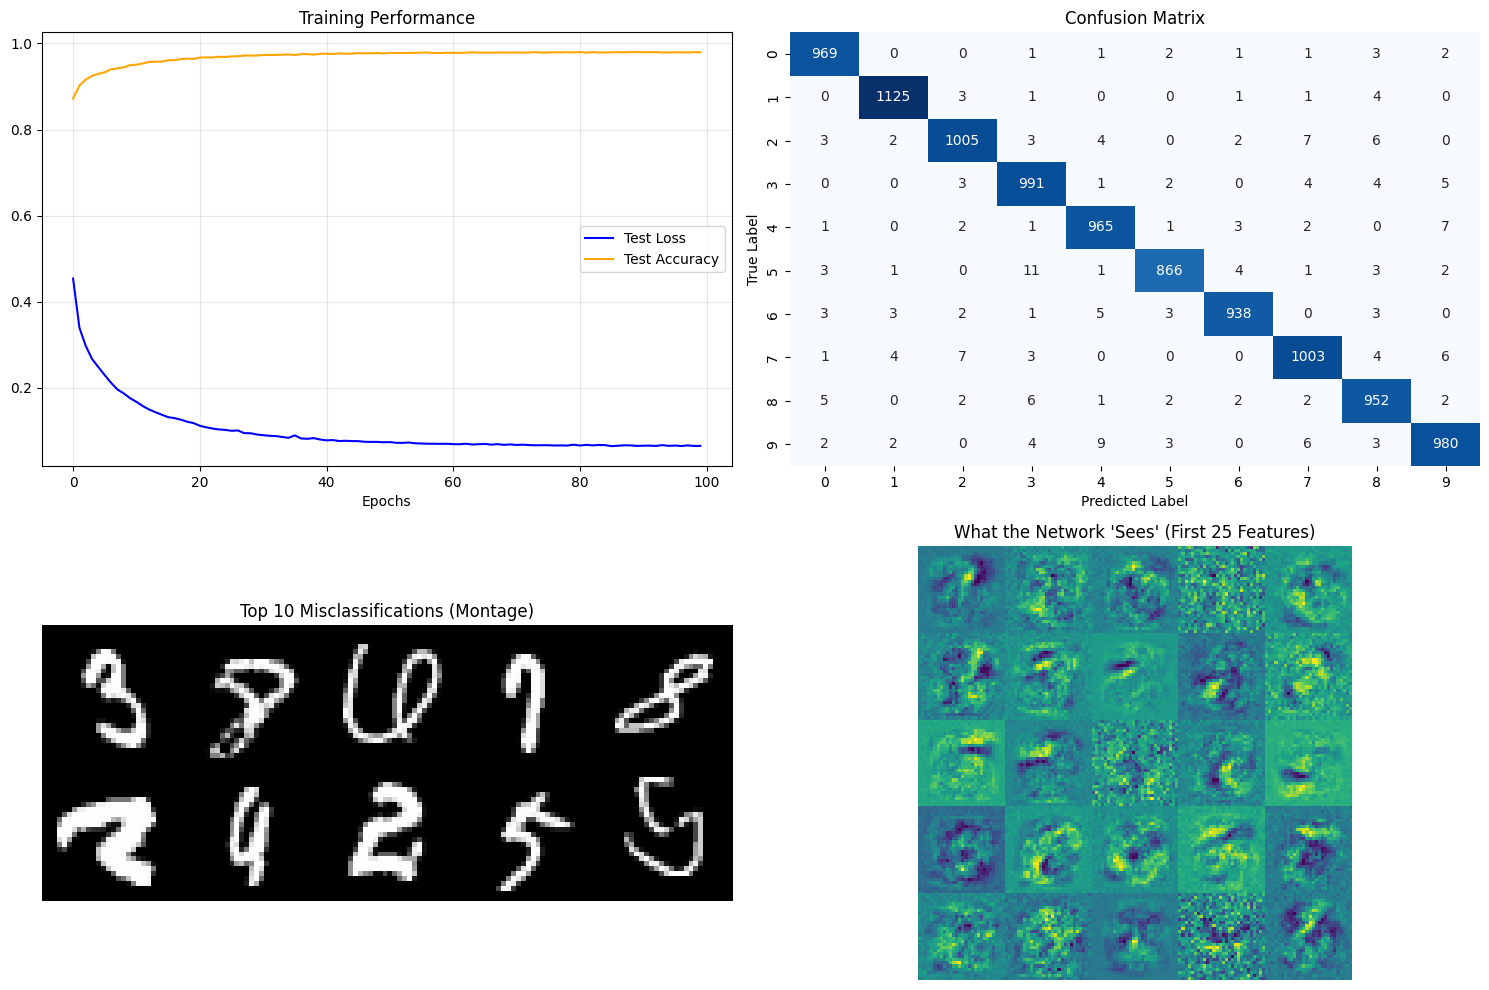
\includegraphics[width=0.95\textwidth]{../results/figures/04_mlp/weight_templates.png}
  \caption{Manual MLP diagnostics from my run: loss/accuracy curves, confusion matrix, and first-layer filters.}
  \label{fig:mlp}
\end{figure}

Table~\ref{tab:cls} summarises the classification ladder through the manual notebooks and the standalone CNN.

\begin{table}[H]
  \centering
  \caption{Classification metrics from saved notebook outputs (\texttt{results/metrics/classification.json}).}
  \label{tab:cls}
  \begin{tabular}{@{}lll@{}}
    \toprule
    Model & Test accuracy & Source notebook \\
    \midrule
    KNN (GPU, $k{=}3$) & 0.9705 & \texttt{manual\_knn.ipynb} \\
    Logistic regression & 0.9241 & \texttt{manual\_logistic\_reg.ipynb} \\
    Manual MLP & 0.9794 & \texttt{manual\_mlp.ipynb} \\
    SimpleCNN & 0.9871 & \texttt{cnn.ipynb} \\
    Comparison CNN & 0.9913 & \texttt{02\_mnist\_models.ipynb} \\
    \bottomrule
  \end{tabular}
\end{table}

\section{CNN baseline}
\label{sec:cnn}

\texttt{cnn.ipynb} implements a small \texttt{SimpleCNN}: two convolutional layers, max pooling, and two linear layers, trained five epochs with SGD. Test accuracy reaches \textbf{0.9871} by epoch 4. The jump from manual MLP to CNN is modest in absolute terms on MNIST, but I think the spatial inductive bias matters: convolutions reuse filters across the image instead of treating every pixel independently.

Figure~\ref{fig:cnn-panel} shows my post-training analysis panel (confusion matrix, ROC-style curves, per-class behaviour). Figure~\ref{fig:filters} visualises first-layer conv filters---mostly edge and blob detectors, which matches what I expected from coursework examples.

\begin{figure}[H]
  \centering
  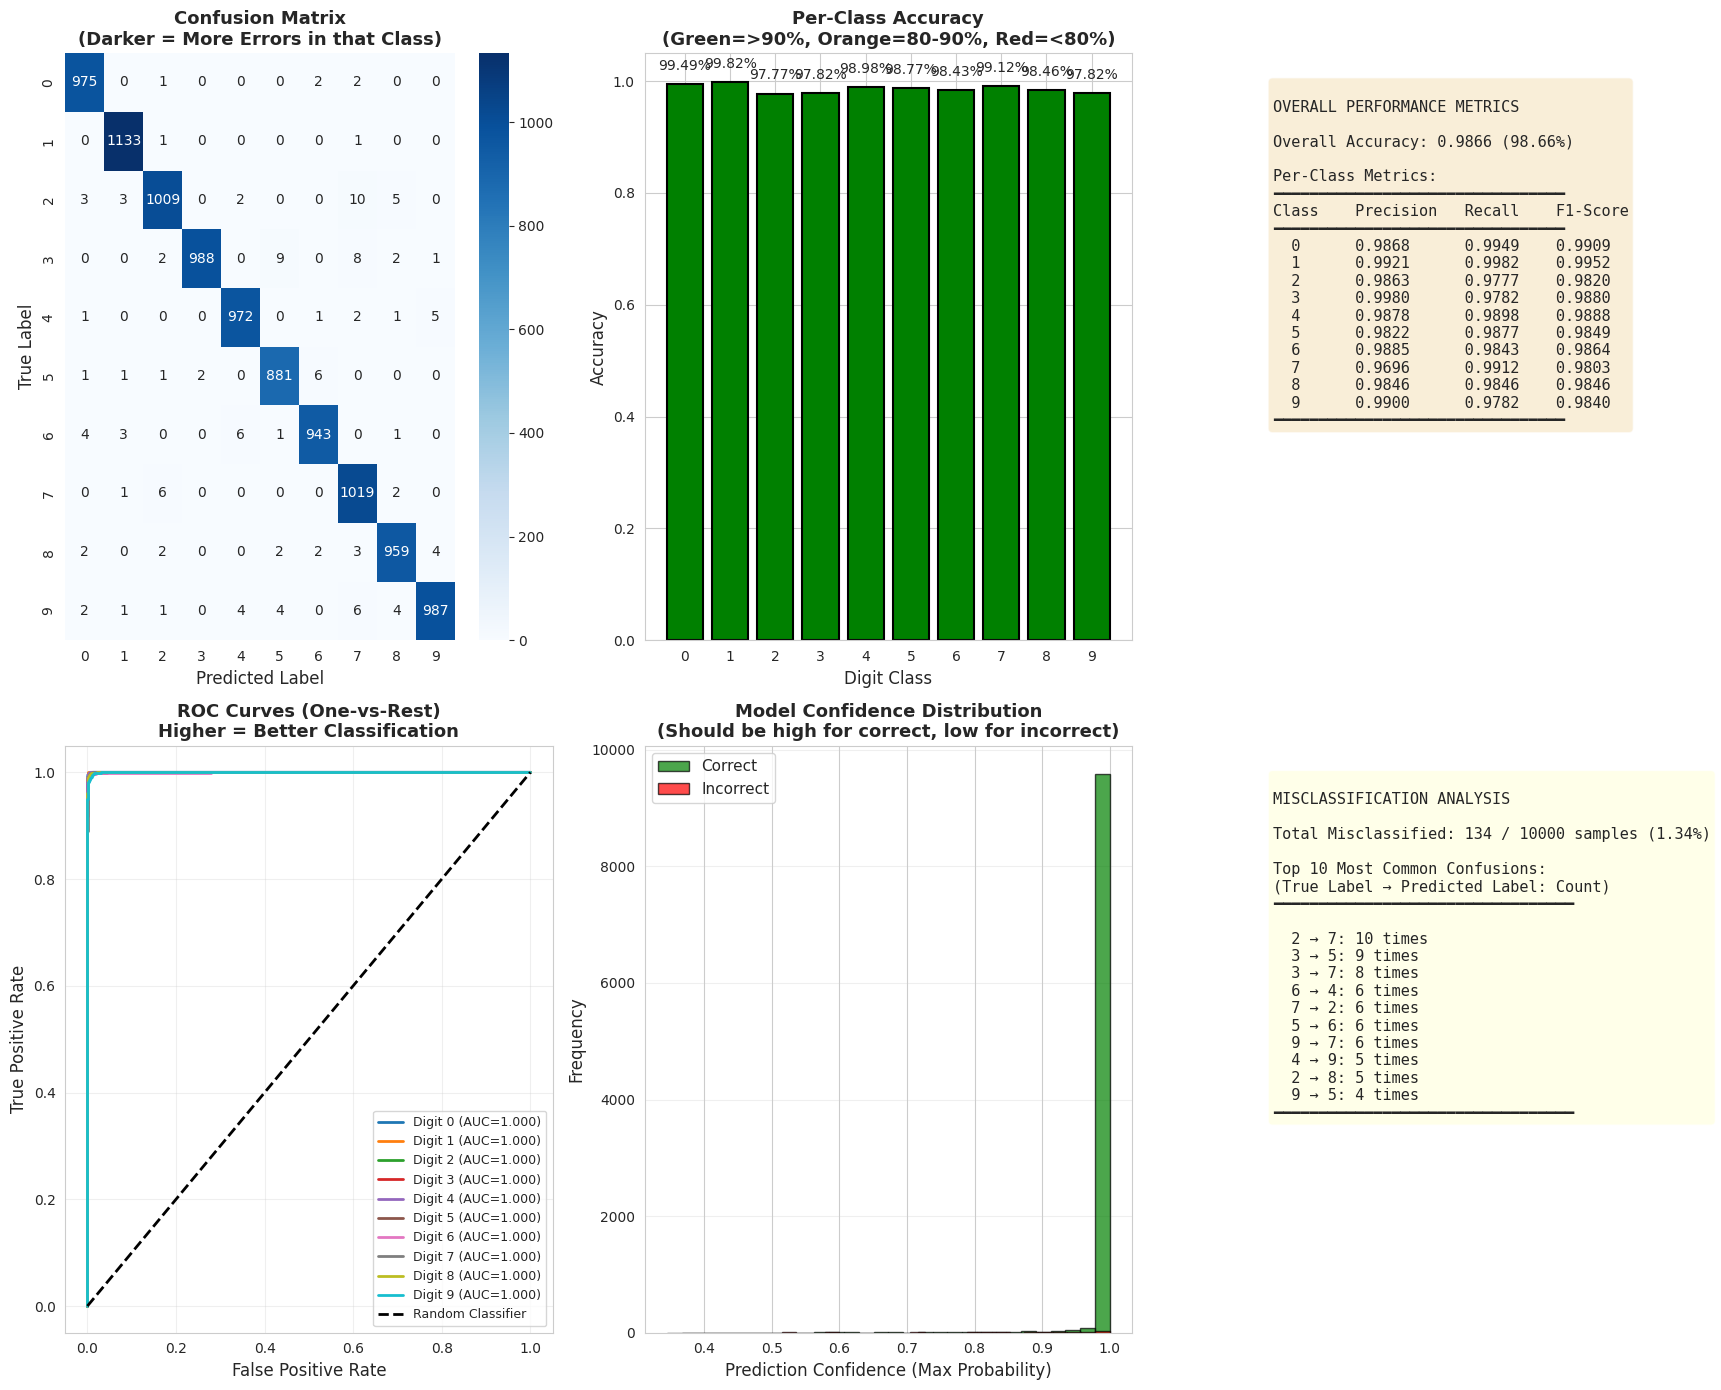
\includegraphics[width=0.98\textwidth]{../results/figures/05_cnn/confusion_matrix.png}
  \caption{CNN evaluation panel from my saved run (confusion matrix and ROC-related plots in one figure).}
  \label{fig:cnn-panel}
\end{figure}

\begin{figure}[H]
  \centering
  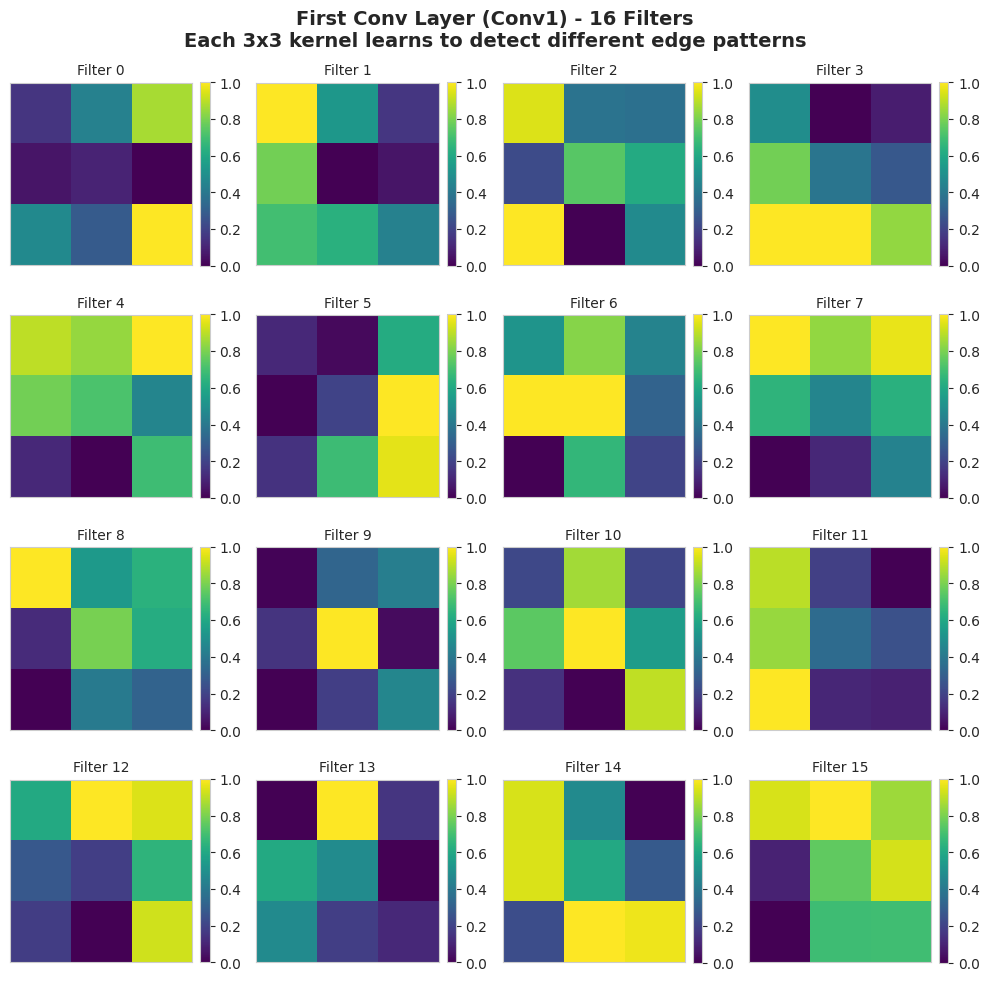
\includegraphics[width=0.75\textwidth]{../results/figures/05_cnn/conv_filters.png}
  \caption{Learned filters in the first convolutional layer.}
  \label{fig:filters}
\end{figure}

\section{Generative models}
\label{sec:gen}

After classification, I worked through four generative approaches in increasing complexity. I did not run FID or IS; I judged samples by eye on the PNG grids in \texttt{results/figures/}.

\subsection{Variational autoencoder}

\texttt{vae.ipynb} trains a convolutional VAE with a 16-D latent space for 50 epochs. Final train/validation total loss is \textbf{100.22 / 100.09} (reconstruction plus weighted KL). Reconstructions (Figure~\ref{fig:vae-recon}) preserve digit identity but look soft, which is what I usually see with Bernoulli/BCE or MSE-style decoders on MNIST.

\begin{figure}[H]
  \centering
  \begin{subfigure}[b]{0.48\textwidth}
    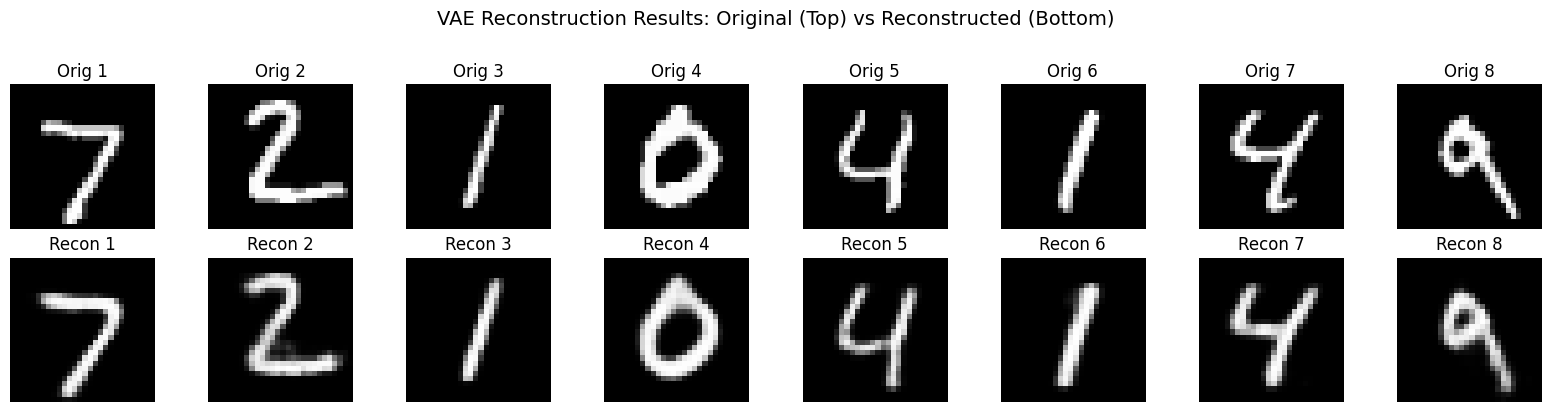
\includegraphics[width=\textwidth]{../results/figures/07_vae/reconstructions.png}
    \caption{Reconstructions}
    \label{fig:vae-recon}
  \end{subfigure}
  \hfill
  \begin{subfigure}[b]{0.48\textwidth}
    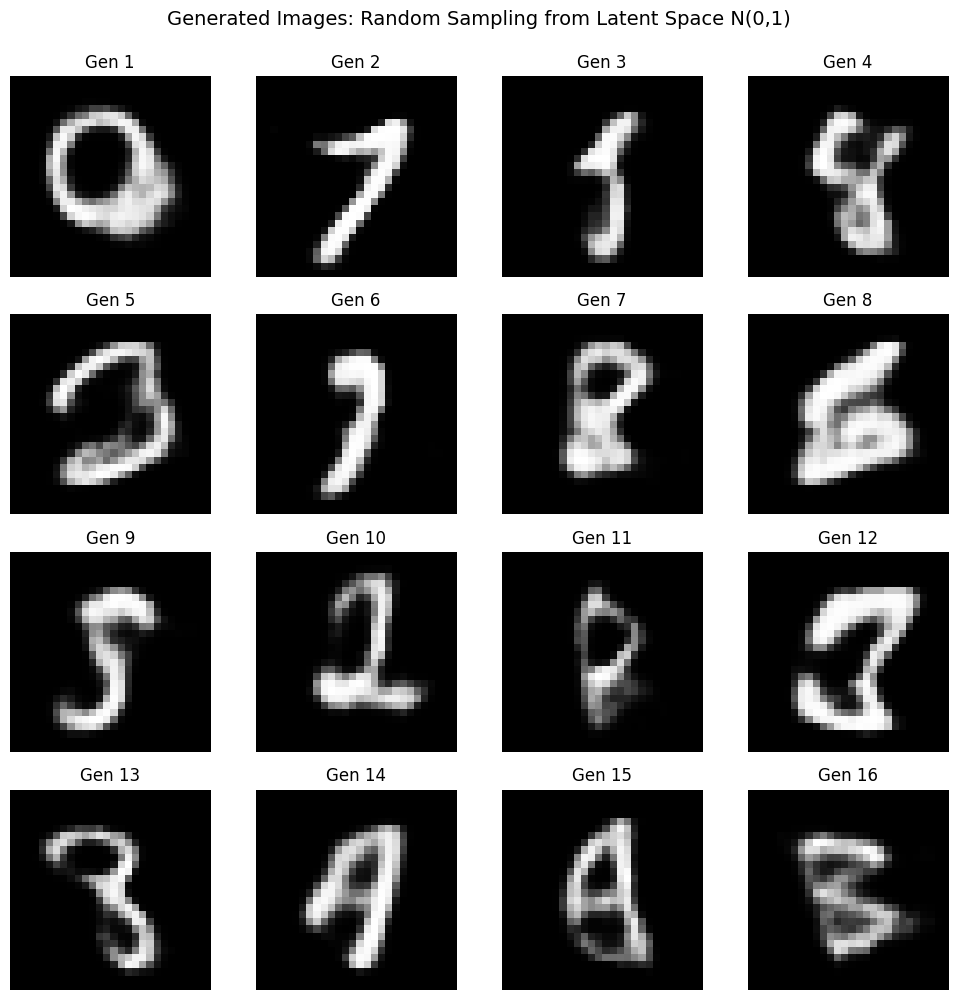
\includegraphics[width=\textwidth]{../results/figures/07_vae/training_curves.png}
    \caption{Training curves}
    \label{fig:vae-train}
  \end{subfigure}
  \caption{VAE outputs from \texttt{vae.ipynb}.}
  \label{fig:vae}
\end{figure}

\subsection{Pixel-space DDPM}

\texttt{ddpm.ipynb} implements a DDPM~\citep{ho2020ddpm} with $T{=}300$ timesteps and a U-Net denoiser, trained 15 epochs. Average loss at epoch 15 is \textbf{0.0454} (Figure~\ref{fig:ddpm-loss}). Generated samples (Figure~\ref{fig:ddpm-grid}) look like MNIST digits on inspection, though training in full 784-D pixel space felt slower and heavier than the latent diffusion stage later.

\begin{figure}[H]
  \centering
  \begin{subfigure}[b]{0.48\textwidth}
    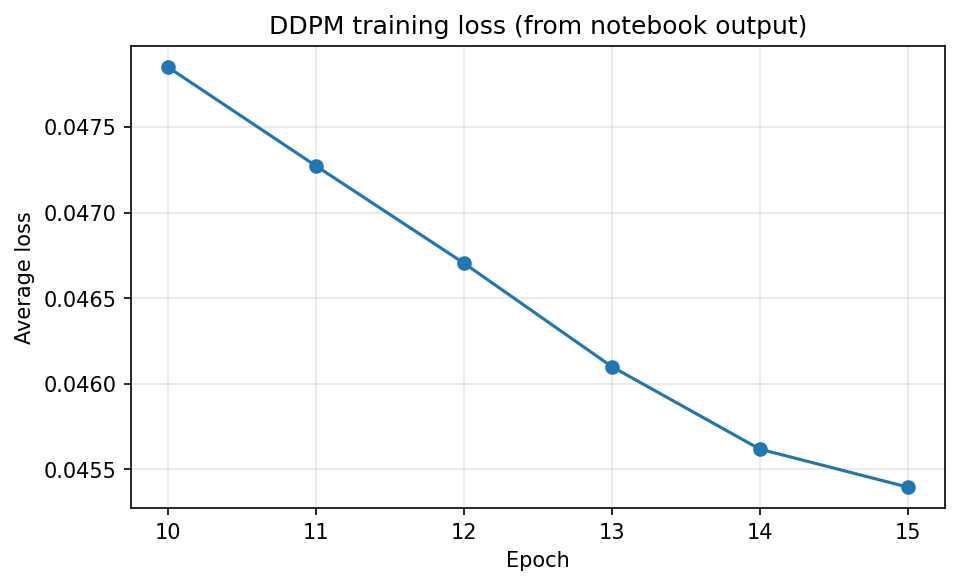
\includegraphics[width=\textwidth]{../results/figures/08_ddpm/loss_curve.png}
    \caption{Loss curve (reconstructed from epoch logs)}
    \label{fig:ddpm-loss}
  \end{subfigure}
  \hfill
  \begin{subfigure}[b]{0.48\textwidth}
    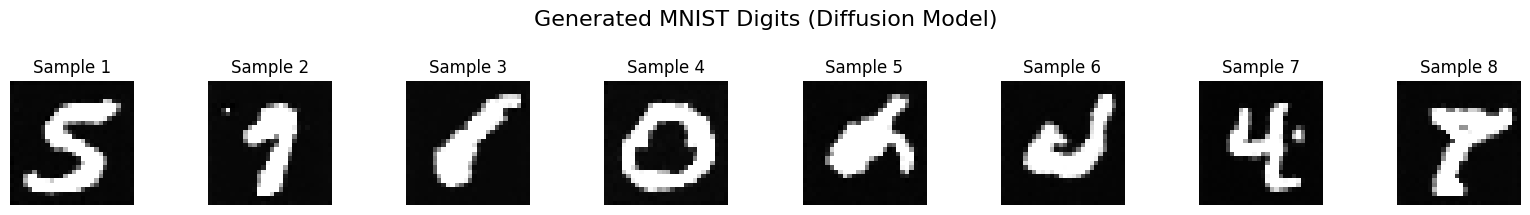
\includegraphics[width=\textwidth]{../results/figures/08_ddpm/denoising_grid.png}
    \caption{Sample grid}
    \label{fig:ddpm-grid}
  \end{subfigure}
  \caption{DDPM training and samples from my notebook outputs.}
  \label{fig:ddpm}
\end{figure}

\subsection{DCGAN}

\texttt{dcgan.ipynb} trains a DCGAN~\citep{radford2016dcgan} for 50 epochs. Final generator/discriminator losses are \textbf{3.41 / 0.32}. The sample grid (Figure~\ref{fig:dcgan}) shows recognisable digits; interpolation (Figure~\ref{fig:dcgan-interp}) suggests the latent space is at least locally smooth. I would not call GAN training ``stable'' here---the loss balance moved around---but the saved outputs are usable for demonstration.

\begin{figure}[H]
  \centering
  \begin{subfigure}[b]{0.48\textwidth}
    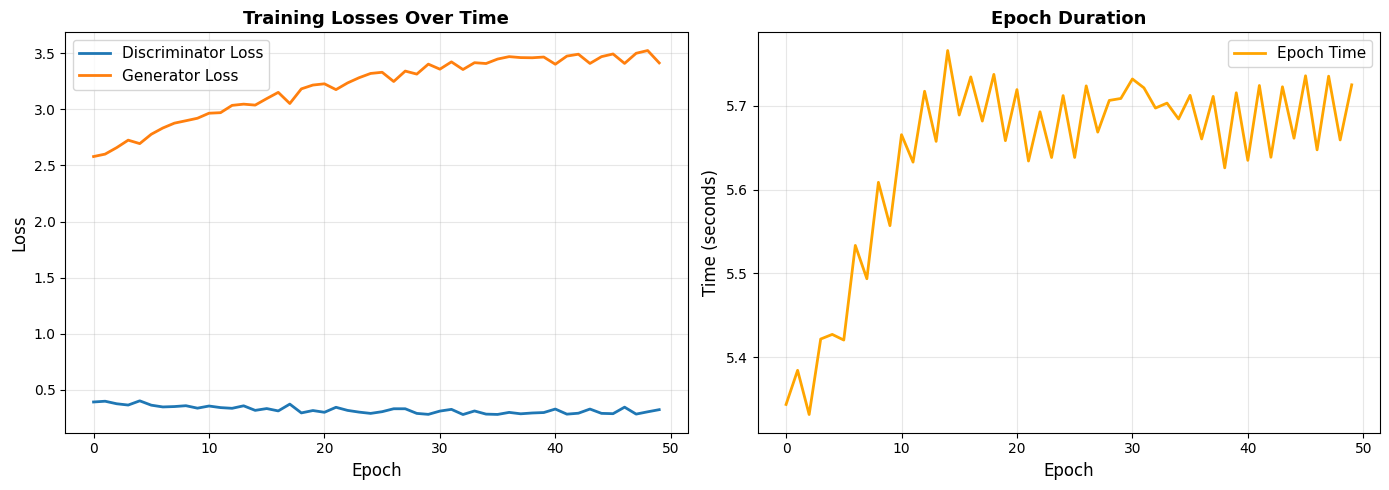
\includegraphics[width=\textwidth]{../results/figures/09_dcgan/generated_digits.png}
    \caption{Generated digits}
    \label{fig:dcgan}
  \end{subfigure}
  \hfill
  \begin{subfigure}[b]{0.48\textwidth}
    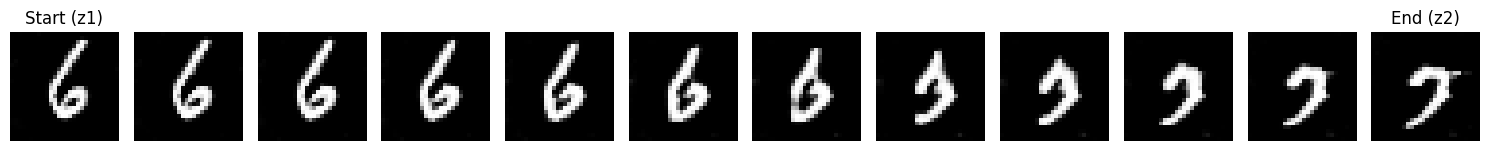
\includegraphics[width=\textwidth]{../results/figures/09_dcgan/latent_interpolation.png}
    \caption{Latent interpolation}
    \label{fig:dcgan-interp}
  \end{subfigure}
  \caption{DCGAN outputs from my saved run.}
  \label{fig:dcgan-all}
\end{figure}

\subsection{Latent diffusion MLP}

The notebook \texttt{vae + 1d unet (latent diff) (1).ipynb} retrains a VAE, extracts latents, and trains a \texttt{LatentDiffusionMLP} for 150 epochs (MSE \textbf{0.224} near the end). Despite ``1d unet'' in the filename, the denoiser is an MLP, not a U-Net---a naming mistake I should fix. Figure~\ref{fig:latent} shows reconstructions and generated samples from that notebook. Functionally, this is the pattern I later used on CIFAR at larger scale: compress first, diffuse second.

\begin{figure}[H]
  \centering
  \begin{subfigure}[b]{0.48\textwidth}
    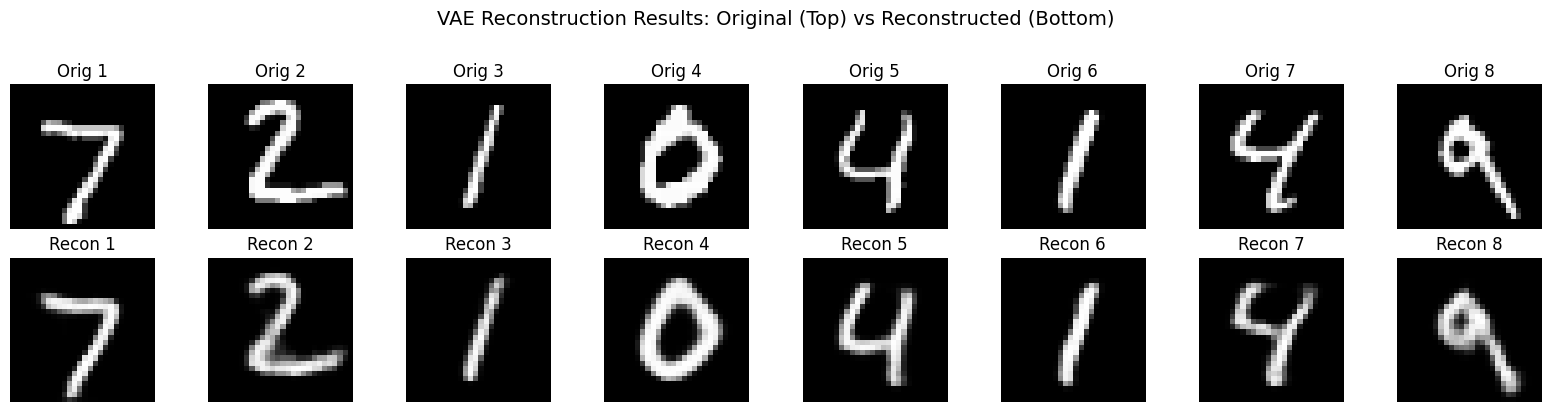
\includegraphics[width=\textwidth]{../results/figures/10_latent_diff/vae_reconstructions.png}
    \caption{VAE reconstructions (latent-diff notebook)}
  \end{subfigure}
  \hfill
  \begin{subfigure}[b]{0.48\textwidth}
    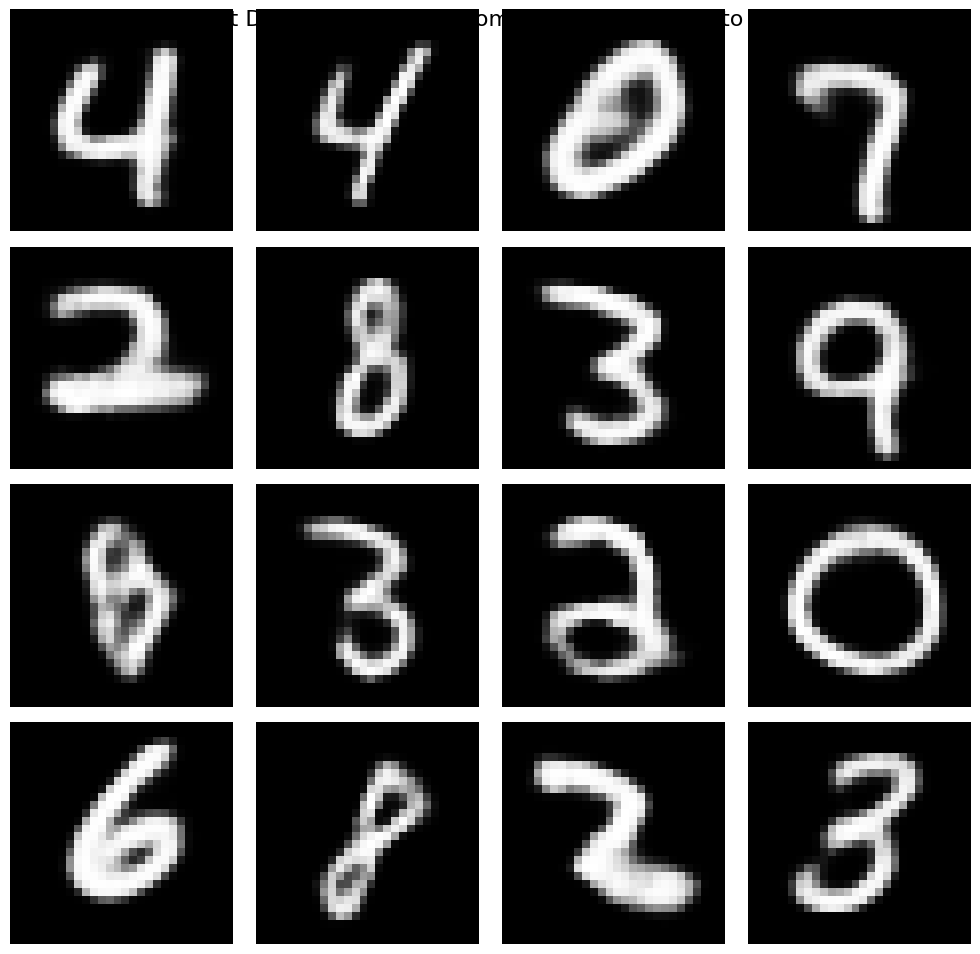
\includegraphics[width=\textwidth]{../results/figures/10_latent_diff/diffusion_samples.png}
    \caption{Latent diffusion samples}
    \label{fig:latent}
  \end{subfigure}
  \caption{Latent diffusion track. Samples are digit-like on visual inspection; sharpness is limited by the VAE bottleneck.}
\end{figure}

\section{Comparison and insights}
\label{sec:compare}

\texttt{02\_mnist\_models.ipynb} benchmarks dummy, sklearn, and PyTorch models on a shared harness. The sorted accuracy bar chart (Figure~\ref{fig:bar}) makes the ladder obvious: deep learning wins on MNIST, but classical KNN is already strong, and the gap from MLP to CNN is incremental rather than dramatic. The comparison CNN reaches \textbf{0.9913}; remaining errors cluster on visually similar pairs (Figure~\ref{fig:conf-pairs}).

\begin{figure}[H]
  \centering
  \begin{subfigure}[b]{0.48\textwidth}
    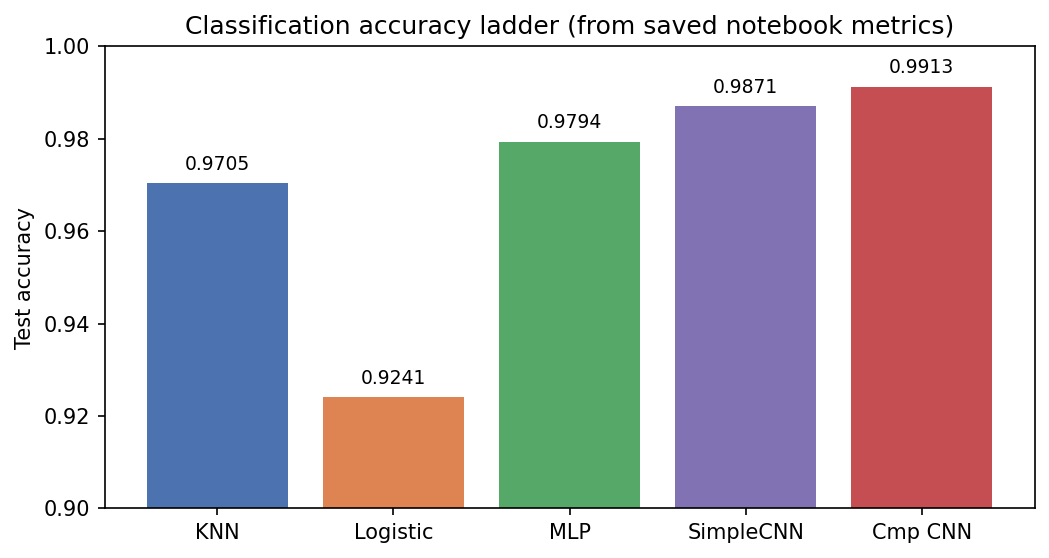
\includegraphics[width=\textwidth]{../results/figures/06_comparison/results_bar_chart.png}
    \caption{Accuracy ladder (from collated metrics)}
    \label{fig:bar}
  \end{subfigure}
  \hfill
  \begin{subfigure}[b]{0.48\textwidth}
    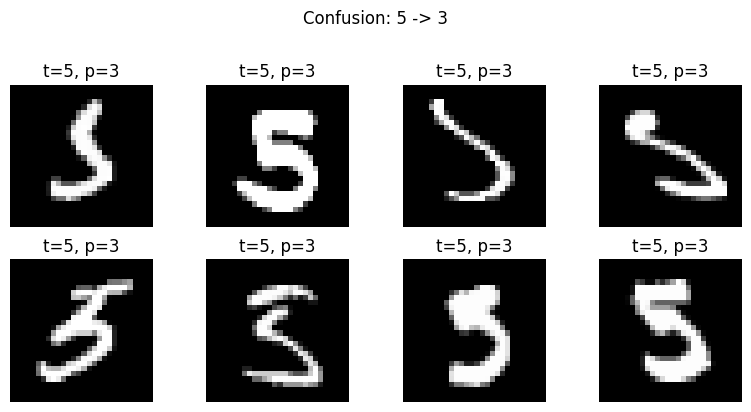
\includegraphics[width=\textwidth]{../results/figures/06_comparison/cnn_confusion_pairs.png}
    \caption{Top CNN confusion pairs}
    \label{fig:conf-pairs}
  \end{subfigure}
  \caption{Multi-model comparison insights from my saved outputs.}
\end{figure}

On the generative side, I think of the tradeoffs this way: VAEs give cheap latent codes but blurry decoders; pixel DDPMs are faithful to the DDPM math but expensive in 784-D; GANs can look sharp but need careful monitoring; latent diffusion is efficient once latents exist but inherits VAE quality. I did not run controlled ablations to rank them quantitatively.

\section{Limitations}
\label{sec:limits}

\begin{itemize}[noitemsep]
  \item \textbf{No FID / IS.} I did not compute standard generative metrics. Claims about sample quality are qualitative.
  \item \textbf{28$\times$28 grayscale only.} Findings may not transfer to colour or high-resolution data.
  \item \textbf{Duplicate VAE training.} \texttt{vae.ipynb} and the latent-diffusion notebook both train a VAE; I should load a checkpoint instead of retraining.
  \item \textbf{Misleading filename.} The latent-diffusion notebook name references a 1D U-Net; the implementation is an MLP.
  \item \textbf{Notebook hygiene.} \texttt{02\_mnist\_models.ipynb} may list duplicate CNN rows from re-runs; I cite \textbf{0.9913} as the comparison result.
  \item \textbf{Reproducibility.} \texttt{requirements.txt} does not pin versions; I relied on embedded outputs as the documentation source of truth.
\end{itemize}

\section{Future work}

\begin{itemize}[noitemsep]
  \item Deduplicate the VAE pipeline (train once, load \texttt{vae\_model.pth} elsewhere).
  \item Add FID or a simple classifier-based generative score.
  \item Rename the latent-diffusion notebook and guard Colab-only cells for local runs.
  \item Extend the same notebook structure to Fashion-MNIST.
  \item Pin \texttt{torch} and \texttt{tensorflow} versions and add a lightweight \texttt{nbconvert} smoke test in CI.
\end{itemize}

\section{Conclusion}

I built an end-to-end MNIST lab that reads like a course project I actually ran: EDA, manual implementations, a CNN benchmark, and four generative families with saved plots in \texttt{results/}. Classification reaches \textbf{0.9913} on the comparison CNN; generative models produce inspectable digit samples without me claiming state-of-the-art numbers. I think documenting the logistic-regression dip, the soft VAE reconstructions, and the missing FID metrics is as important as listing the peak accuracies---it makes the repo credible for someone reviewing my work.

\bibliographystyle{plainnat}
\bibliography{references}

\end{document}
